\section{Постановка задачи машинного обучения}

Одним из первых, кто дал определение предмету машинного обучения стал американский ученый Артур Самуэль. В 1959 году в своей работе \cite{Samuel:ML}, посвященной созданию искусственного интеллекта по игре в шашки с помощью алгоритма minimax, Артур Самуэль дал определение тому, что есть машинное обучение - процесс обучения, в результате которого компьютеры способны показывать поведение, которое в них явно не было заложено.

Более современное и точное определение дал Том Митчелл в 1998 году. Корректно поставленная задача обучения определяется следующим образом. Говорят, что компьютерная программа обучается на основе опыта E (experience) по отношению к некоторому классу задач T (task) и меры качества P (performance), если качество задач из T измеренное на основе P, улучшается с приобретением опыта E.

Большинство алгоритмов машинного обучения условно можно разбить на 2 класса: обучение с учителем (supervised learning) и обучение без учителя (unsupervised learning).

В алгоритмах обучения с учителем подразумевается обучение на размеченных данных, то есть когда дана матрица, описывающая объекты с помощью признаков (матрица объект-признак) и вектор ответов для каждого объекта. Таким образом методы обучения с учителем можно представлять как функциональную зависимость: на каждый набор признаков $x \in X$ есть ответы $Y$ такой, что $y:~X \rightarrow Y$, где $y$ - искомая зависимость.

Рассмотрим такой подход более подробно \cite{coursera:voroncov}. Пусть $X$ - множество объектов, $Y$ -- множество ответов, $y:~X \rightarrow Y$ -- неизвестная зависимость (target function).

Пусть также нам известны:\\
\begin{description}[font=$\bullet$]
    \item $\{ x_1, \dots, x_l \} \subset X $ -- известное подмножество объектов;\\
    \item $y_i = y(x_i),~~\forall~i=\overline{1,n}$ -- известное множество результатов.\\
\end{description}
Ставится задача найти $a:~X \rightarrow Y$ -- искомый алгоритм (decision function).

Замечание: как правило множество объектов описывается с помощью признаков. Пусть есть $n$ объектов, тогда под признаками объекта будем иметь в виду следующее отображения: $f_j:~X \rightarrow D_j,~~\forall~j=\overline{1,n}$.\\
Признаки могут быть: количественными $D_j=\mathbb{R}$, бинарными $D_j=\{A, B\}$, номинальными $|D_j|=k<\infty$, упорядочено номинальными. Один объект может задаваться набором признаков разных типов.

Тогда объект $x \in X$ может быть описан вектором признаков $f_1(x), \dots, f_n(x)$.
Следовательно, все объекты можно описать с помощью матрицы ''объекты-признаки'' (feature data):
$$ F = 
\begin{pmatrix}
f_1(x_1) & f_2(x_1) & \dots & f_n(x_1) \\
f_1(x_2) & f_2(x_2) & \dots & f_n(x_2) \\
\dots    & \dots    & \dots & \dots    \\
f_1(x_l) & f_2(x_l) & \dots & f_n(x_l) \\
\end{pmatrix}
$$
Каждой строчке соответствуют правильные (ожидаемые) ответы, полученные в результате эксперимента, наблюдения, опроса и т.д. По типу представления множества ответов можно разбить на 3 класса:
\begin{description}[font=$\bullet$]
    \item классификация: $Y=\{A,B\},~Y=\{A_1,\dots,A_k\},~Y\{A,B\}^k$;
    \item регрессия: $Y=\mathbb{R},~Y=\mathbb{R}^k$;
    \item ранжирование: $Y$ -- конечное упорядоченное множество.
\end{description}

Предсказательная модель $a(x)$ строится как параметрическое семейство функций над некоторой фиксированной функцией $g(x)$. Более формально модель $A = \{ a(x) = g(x,\theta) | \theta \in \Theta \}$, где $g:~X \times \Theta \rightarrow Y$ -- фиксированная функция, $\Theta$ -- множество допустимых параметров $\theta$.


В обучении без учителя данные об ответах неизвестны, поэтому можно говорить лишь о том как данные расположены друг относительно друга, данный метод машинного обучения происходит без участия экспериментатора и применяется для обнаружения внутренних взаимосвязей. Обычно так решаются задачи кластеризации, понижения размерности, визуализации данных.

Также используются методы обучения с подкреплением (reinforcement learning), когда набор данных дается из некоторого потока, а также рекомендательные системы (recommender systems).

\section{Методология решения задач машинного обучения}

Вне зависимости от метода машинного обучения задача состоит из 2-х этапов: обучение и применение.
На первой стадии происходит построение оптимального алгоритма $a$ -- функция, дерево, набор инструкций и др. На второй стадии алгоритм выдает ответы для новых объектов.

Оптимальным алгоритмом будем называть такой алгоритм, который на большинстве объектов обучающей выборки дает правильные ответы или достаточно близкие ответы к ожидаемым. Для того чтобы это сделать нужно определять точность или расстояние между объектами, другими словами нужно задать метрику в пространстве объектов. Для этого вводится понятие функции потерь $\mathfrak{L}$ -- величина ошибки алгоритма $a \in A$ на объекте $x \in X$:
\begin{description}[font=$\bullet$]
    \item $\mathfrak{L} (a,x)=[a(x) \neq y(x)]$ -- индикатор ошибки для случая классификации;
    \item $\mathfrak{L} (a,x)= (a(x) - y(x))^p$ -- для случая регрессии.
\end{description}
Замечание: при $p=1$ для регрессии функция ошибки берется как модуль разности алгоритма и ответа.

На практике для случая регрессии обычно берут $p=2$ т.к. при $p=1$ возникает проблема с дифференцированием функции потерь. 

Чтобы оценить алгоритм в целом берут деленную на размер сумму функций потерь, получившуюся величину называют эмпирическим риском (функционал качества алгоритма $a$ на объектах $X^l$): $Q(a, X^l) = \dfrac{1}{l}\sum\limits_{i=1}^{l}\mathfrak{L}(a,x_i)$.

Таким образом задача обучения сводится к задаче оптимизации (минимизация эмпирического риска на обучающей выборке): $\mu(X^l) = \arg\min\limits_{a \in A} Q(a,X^l)$.

Для решения задачи минимизации применяют различные численные методы. Например, метод наименьших квадратов (МНК).


\subsection{CRISP-DM}

\begin{wrapfigure}{r}{0.44\linewidth} 
    \vspace{-5ex}
    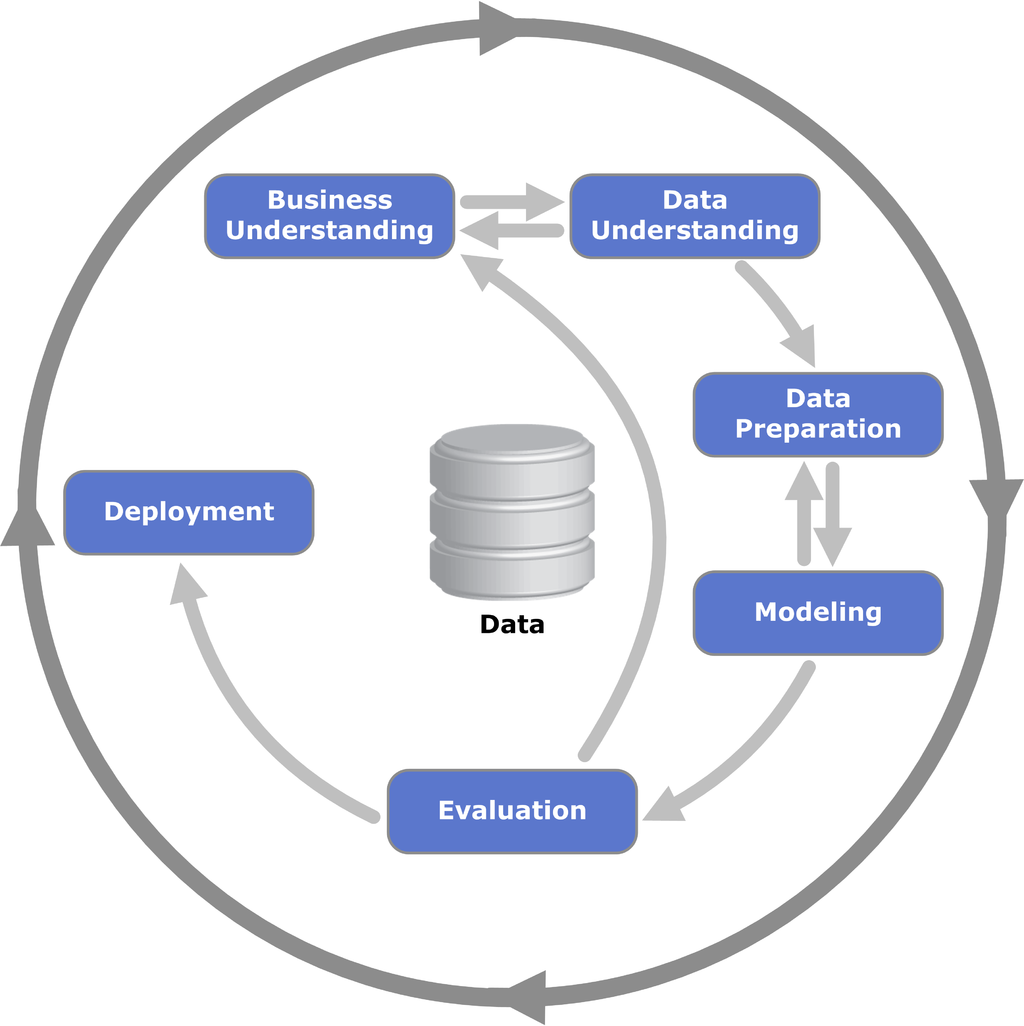
\includegraphics[width=\linewidth]{src/img/CRISP-DM_process_diagram.png}
    \caption{Жизненный цикл исследования данных \cite{wiki:crisp_dm}}
    \label{fig:crisp_dm}
\end{wrapfigure}

Таким образом, любая задача машинного обучения: классификация, регрессия, кластеризация сводится к оптимизационной задаче. Что приводит к большому множеству методов машинного обучения, чтобы облегчить процесс решения задач, был разработан CRISP-DM (CRoss Industry Standard Process for Data Mining) -- межотраслевой стандарт решения задач интеллектуального анализа данных. CRISP-DM -- модель жизненного цикла исследования данных.
Первая версия данного стандарта была принята в 1999 году. Стандарт призван формализовать схему решения задач анализа данных. Предполагается решение любой задачи в 5 шагов, причем они могут замыкаться в цикле. 

\begin{enumerate}[label=\arabic*.]
    \item В начале исследователь должен понять предметную область или сферу бизнеса;
    \item Далее необходимо понять как собирались данные;
    \item На следующем шаге нужно определить есть ли в данных шумы, пропуски, выбросы, все ли признаки несут полезную информацию, можно ли вычислить полезные признаки по уже имеющимся, данный этап можно назвать подготовкой данных;
    \item После происходит моделирование или построение предсказательной модели;
    \item Полученная модель оценивается с помощью выбранных метрик;
    \item Если качество полученной модели удовлетворяют исследователя, модель внедряется в производственные процессы и эксплуатируется.
\end{enumerate}
Помимо CRISP-DM существуют менее известные стандарты: My own, SEMMA и другие. На сайте \cite{poll:crisp_dm} публикуются результаты опросов по популярности методологий анализа данных.

\section{Регрессионный анализ}


\subsection{Линейные модели}

\subsubsection{Линейная регрессия}

\subsubsection{Полиномиальная регрессия}

\subsubsection{Пуассоновская регрессия}

\subsubsection{Геометрическая регрессия}

\subsubsection{Проблема переобучения}

Пример линейной модели\\

Эмпирические оценки обобщающей способности\\
* Эмпирический риск на тестовых данных (Hold-out)\\
* Скользящий контроль (leave-one-out)\\
* Кросс-проверка (cross-validation) по N разбиениям\\

\subsection{Нелинейные модели}

\subsubsection{Градиентный бустинг}

\subsubsection{Решающие деревья}

\subsubsection{Случайный лес}
